\documentclass{slide}
\usepackage{tikz}

\title{Introduction}
\subtitle{Software Architecture}
\institute{University of Queensland}
\author{Richard Thomas}
\date{\week{1}}
\titlegraphic {
    \begin{tikzpicture}[overlay,remember picture]
    \node[left=0.1cm] at (current page.-9){
        \href{https://xkcd.com/2347/}{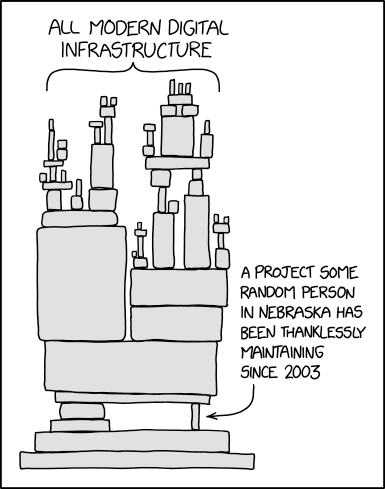
\includegraphics[width=4.75cm]{images/dependency.png}}
    };
    \end{tikzpicture}
}

\begin{document}

\maketitle

\question{What is \highlight{Software Architecture}?}

\point{\highlight{Software Architecture} is design.\\~\\
\highlight{Design} is not software architecture.
}

\point[But...]{\highlight{Software Architecture} is hard to define.}

\point[Let's hear from an expert]{\centering \youtubevideo{images/making-architecture-matter-thumb}{https://www.youtube.com/watch?v=DngAZyWMGR0}}

\definition[Okay so...]{Software Architecture}{The important stuff; whatever that is.}

\question{What do \highlight{you} want from this course?}

\definition[Maybe...]{Software Architecture: The Course}%
{A set of tools, processes, and design patterns which enable me to deliver high quality software.}


\begin{frame}{High Quality Software?\footnote{Yes, ``high quality'' is intentionally vague.}}

\Large{
\begin{description}
    \setlength\itemsep{0.5em}
    \item[Functional Requirements] -- Functional features to be delivered.
    \item[Constraints] -- Real world constraints on development.
    \item[Principles] -- Ideas adopted to encourage design consistency.
    \item[Quality Attributes] -- Quality of service and cross-cutting concerns.
\end{description}
}

\end{frame}


\begin{frame}{Functional Requirements}

\Large{
\begin{itemize}
    \item Architecture must enable delivery of functionality.
	\vspace{0.3em}
    \item Support interaction model.
    \begin{itemize}
        \large{\item[$\bullet$] A mobile dating app may be difficult to deliver using \highlight{Pipe and Filter}.}
    \end{itemize}
	\vspace{0.3em}
    \item Don't over architect.
    \begin{itemize}
        \large{\item[$\bullet$] A mobile dating app doesn't need a six-layer \highlight{PCBMER} architecture.}
    \end{itemize}
\end{itemize}
}

\end{frame}


\begin{frame}{Constraints}

\Large{
\begin{itemize}
    \item Externally determined restrictions
	\vspace{0.2em}
    \item Time and budget
	\vspace{0.2em}
    \item Technology
    \begin{itemize}
        \large{\item[$\bullet$] Interoperability with existing systems}
        \large{\item[$\bullet$] Deployment platform}
        \large{\item[$\bullet$] Vendor relationships}
    \end{itemize}
	\vspace{0.2em}
    \item People
	\vspace{0.2em}
    \item Organisation
    \begin{itemize}
        \large{\item[$\bullet$] Strategic or tactical system?}
        \large{\item[$\bullet$] Politics may limit choices}
    \end{itemize}
\end{itemize}
}

\end{frame}


\begin{frame}{Principles}

\Large{
\begin{itemize}
    \item Standards developers are expected to follow
    \begin{itemize}
        \large{\item[$\bullet$] Avoid unintentionally breaking the architecture}
    \end{itemize}
	\vspace{0.3em}
    \item e.g. Architectural structure
    \begin{itemize}
        \large{\item[$\bullet$] Layering strategy}
        \large{\item[$\bullet$] Location of business logic}
        \large{\item[$\bullet$] Stateless components}
    \end{itemize}
\end{itemize}
}

\end{frame}


\questionanswer{What are \highlight{Quality Attributes}?\extra{Hint: CSSE3002 / CSSE3012}}{Non-functional requirements for the success of software.}

\begin{frame}{Quality Attributes: Examples}

\large{
\begin{description}[<+->]
    \setlength\itemsep{0.35em}
    \item[Modularity] Components of the software are separated into \highlight{discrete modules}.
    \item[Availability] The software is \highlight{available to access} by end users, either at any time or on any platform, or both.
    \item[Scalability] The software can handle peaks of high demand by \highlight{taking advantage of available computing resources}.
    \item[Extensibility] Features or extensions can be \highlight{easily added} to the base software.
    \item[Testibility] The software is designed so that \highlight{automated tests} can be easily deployed.
\end{description}
}

\end{frame}


\point[Problem]{Software cannot meet all quality attributes.}

\point[``Solution'']{Software architects prioritise the important attributes.\extra{on a software-by-software basis}}

\definition{The First Law of Software Architecture \cite{richards2020fundamentals}}{Everything in software architecture is a trade-off.}

\definition{Wicked Architecture \cite{wicked-architecture}}%
{There are often \highlight{no clear problem descriptions}, \highlight{no clear solutions},
good or bad solutions, \highlight{no clear rules} when to ``stop'' architecting
and mostly team rather than individual work.\\
\extra{Don't expect ``clean'' solutions.}}

\point[Why now?]{Architecture is more important today thanks to \highlight{expectations} and \highlight{infrastructure}.}

\quote[Dave Thomas]{Big design up front is dumb.\\ \vspace{0.75em}Doing no design up front is even dumber.}

% Move to week 2 notes, prior to security guest lecture.
%\begin{frame}
%
%\begin{figure}
%    \href{https://xkcd.com/2166/}{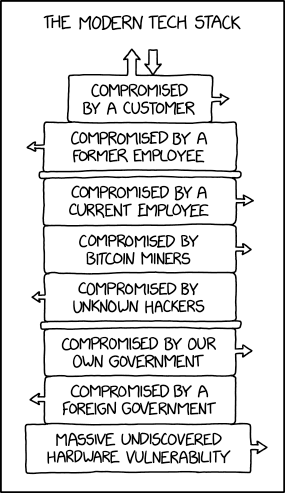
\includegraphics[height=\paperheight-11mm]{images/security_stack.png}}
%    \caption{\url{https://xkcd.com/2166/}}
%\end{figure}
%
%\end{frame}

\references{articles,books}

\end{document}
